Il primo esperimento consiste nello studio del comportamento di un convertitore di tensione switching - SMPC - di tipologia Buck ad \textbf{anello aperto}. Il circuito è rappresentato in Figura \ref{fig:Circuit1}. Sono stati utilizzati i seguenti componenti:
\begin{itemize}
    \item Circuito RLC:
    \subitem Resistenza di carico $R_L=50\Omega$, ottenuta dal parallelo di due resistenze da $100\Omega,1W$
    \subitem Induttore L, scelto tra quelli disponibili in laboratorio.
    \subitem Condensatore C, scelto tra i disponibili in laboratorio.
\end{itemize}
\begin{figure}[H]
    \centering
    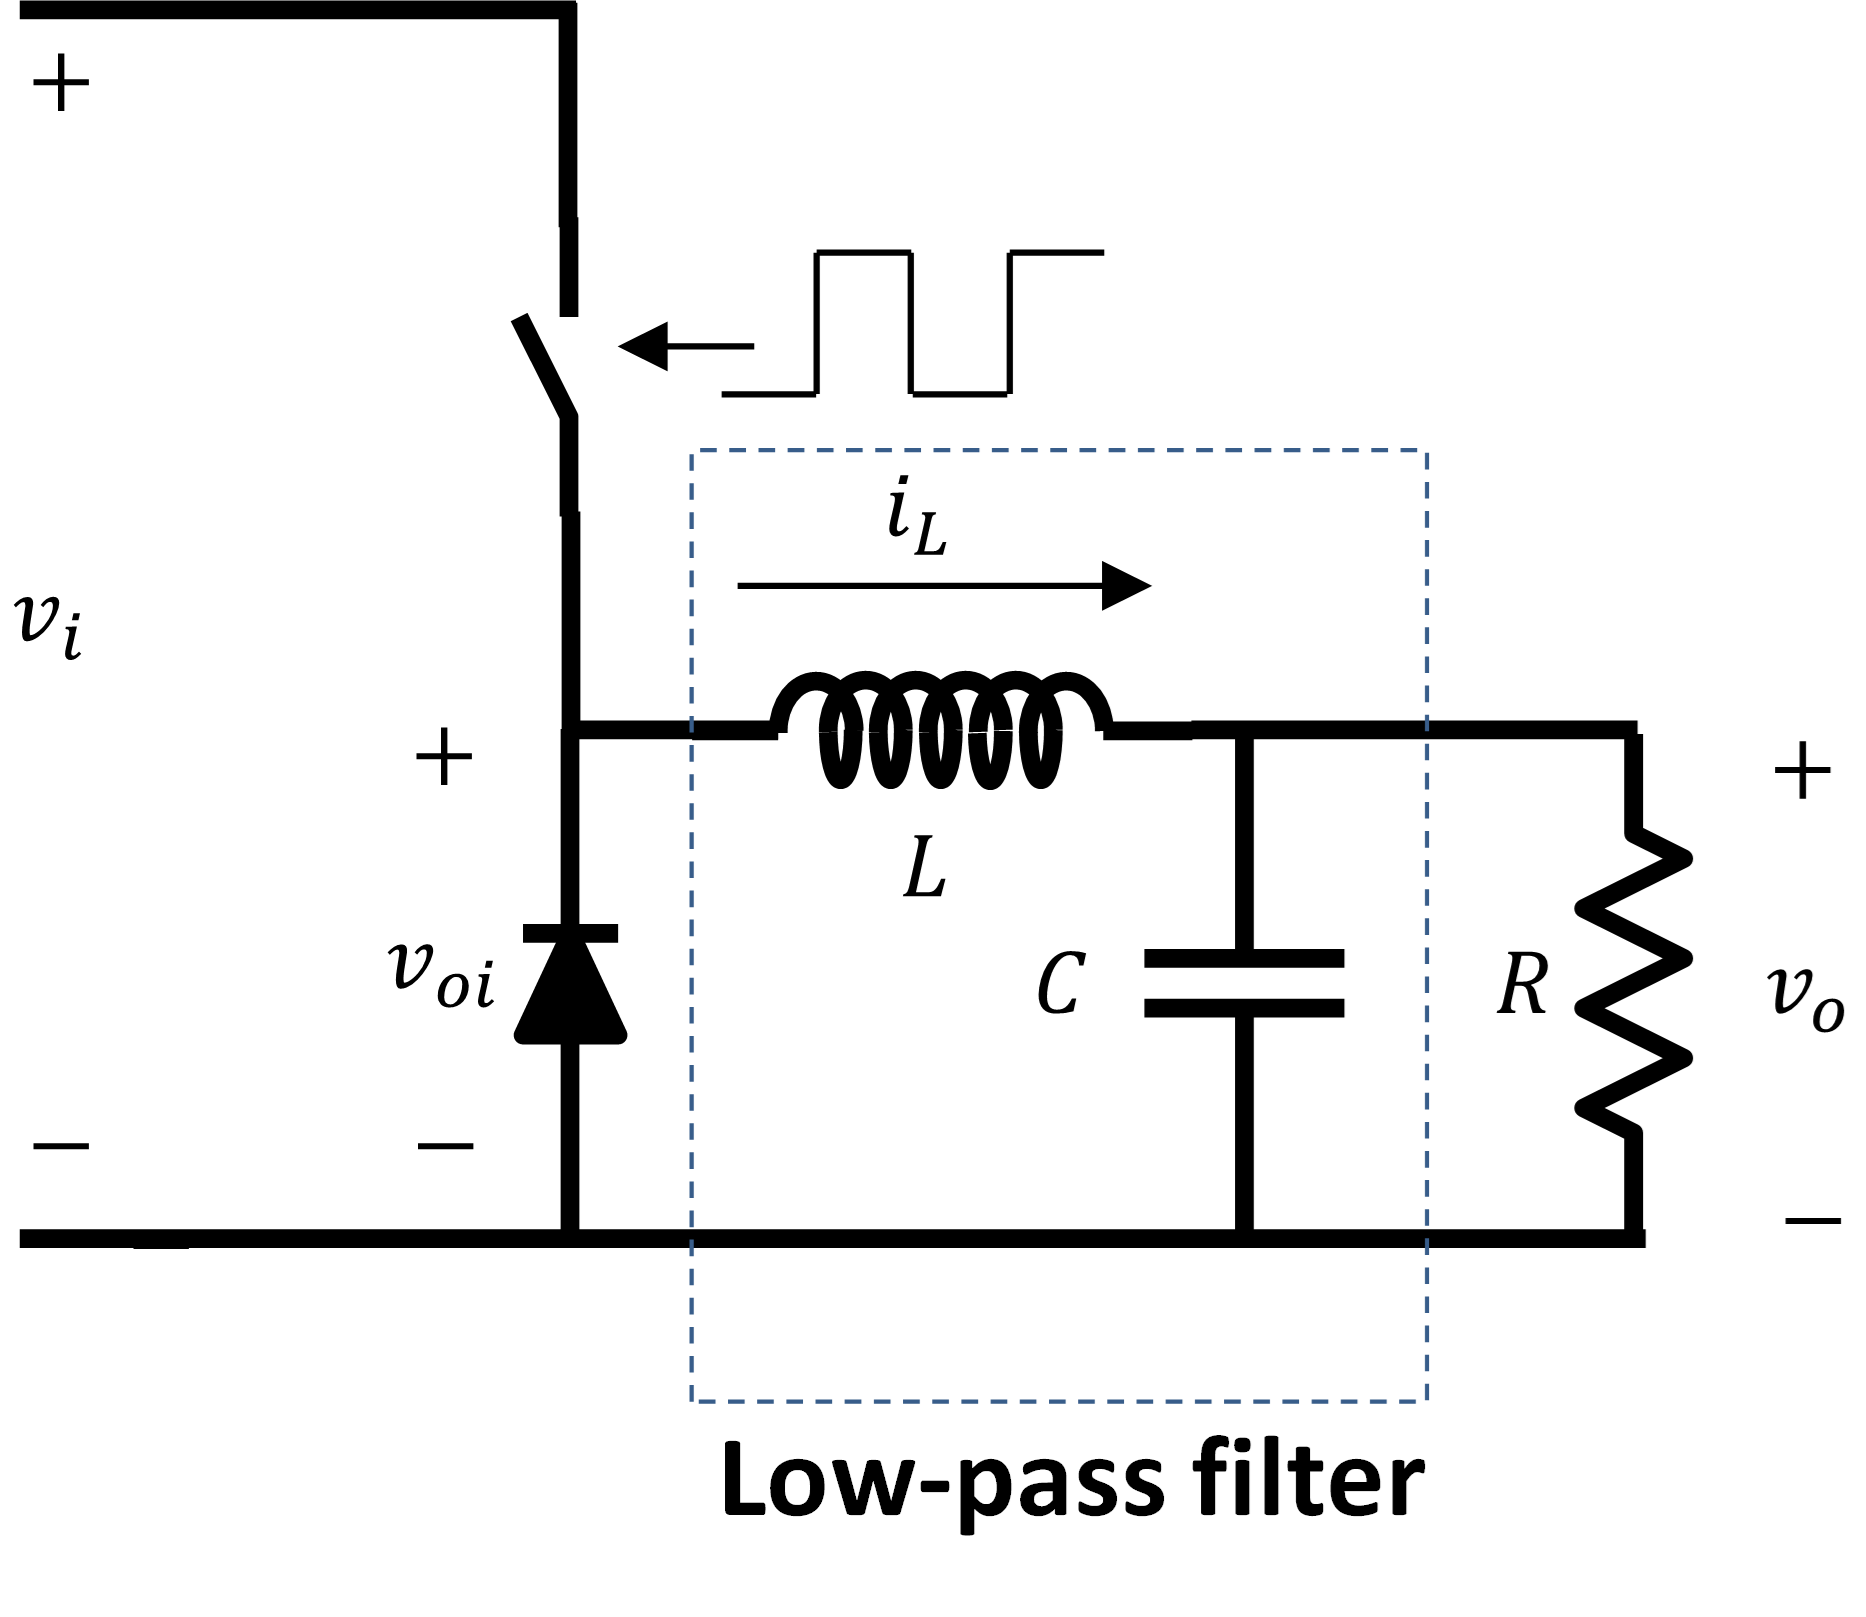
\includegraphics[width=0.5\linewidth]{images/Circuit1.png}
    \caption{Schema circuito}
    \label{fig:Circuit1}
\end{figure}
Il circuito è alimentato dalla tensione $Vi=+8V$.
\subsection{Dimensionamento di \textit{L} e \textit{C} - prelab}\label{ch:Cap1}
Considerata una frequenza di switching di $f=50kHz$ e una tensione di ingresso $V_i=+8V$, si determina il valore minimo dell'induttanza tale da garantire la condizione di \textit{continuos conduction mode} per un  duty cycle maggiore del 20\%. Si vuole quindi che sia garantita la condizione
\begin{equation}
    I_{min}=V_o\left(\frac{1}{R}-\frac{1-\delta}{2L_{min}f}\right)=0\implies L_{min}=\frac{(1-\delta)R}{2f}=400\mu H
\end{equation}
Per cui è stata scelta la seguente induttanza dagli induttori disponibili in laboratorio: $L=680\mu H$.\\\\
Di conseguenza ci si aspetta i seguenti valori per la minima e massima corrente di induzione
\begin{equation}
    I_{Lmax}=V_o\left(\frac{1}{R}+\frac{1-\delta}{2Lf}\right)=50.82mA
\end{equation}
\begin{equation}
    I_{Lmin}=V_o\left(\frac{1}{R}-\frac{1-\delta}{2Lf}\right)=13.18mA
\end{equation}
Successivamente si determina un valore appropriato per il condensatore $C$ tale da garantire che l'output voltage ripple $\Delta V_c$ sia più piccolo di $100mV$. Con l'ausilio della relazione
\begin{equation}
    C=\frac{\Delta I_L}{8f\Delta V_c}\implies C=0.5881\mu F
\end{equation}
è stato scelto il seguente valore per la capacità $C=1\mu F$.





\subsection{Assemblaggi e settaggi}
Dopo aver assemblato il circuito, seguendo lo schematico in Figura \ref{fig:Circuit1SPICE}. Il circuito è stato alimentato utilizzando il canale 2 dell'alimentatore da banco, impostato in modo da erogare la tensione di $V_i=+8V$.
\begin{figure}[H]
    \centering
    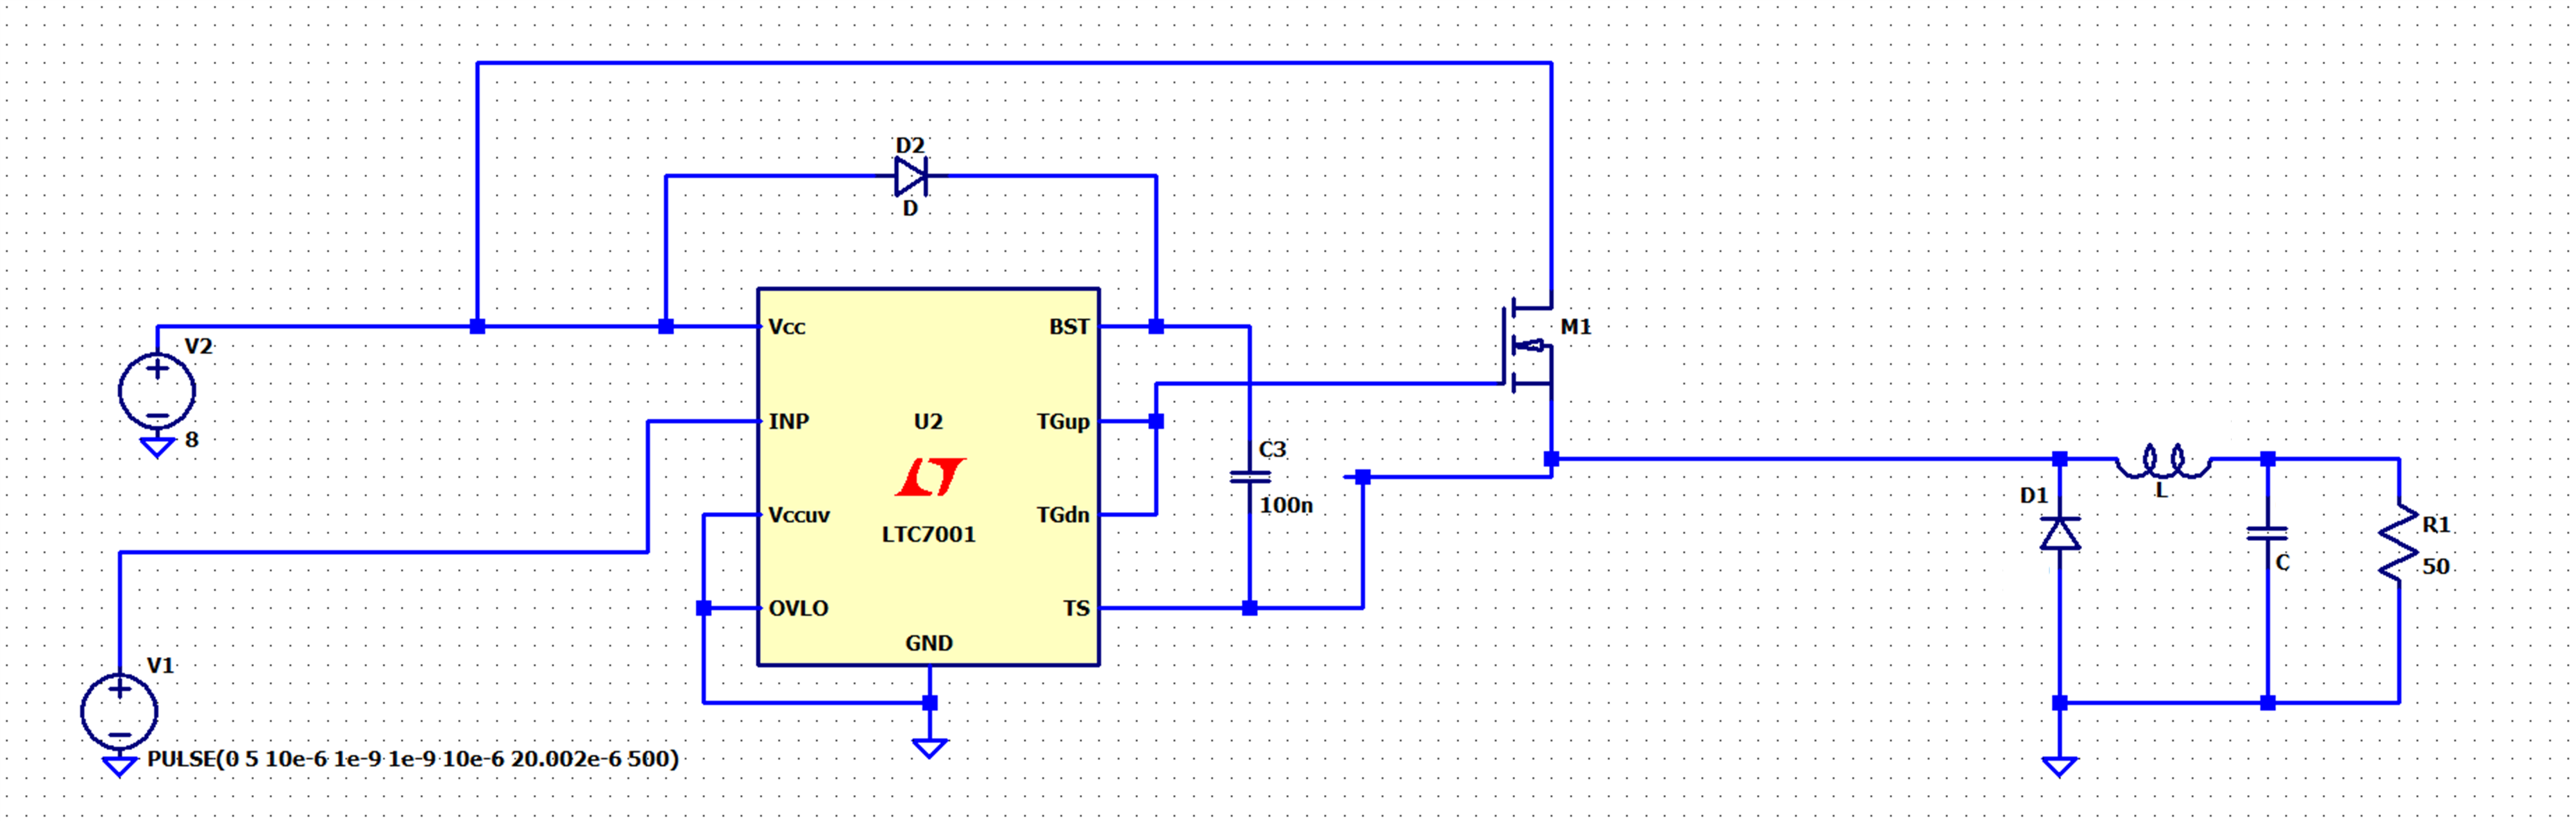
\includegraphics[width=\linewidth]{images/Circuit1SPICE.png}
    \caption{Schematico SPICE del circuito}
    \label{fig:Circuit1SPICE}
\end{figure}
Tramite il generatore di funzioni è stato fornito al terminale \textit{INP} dell' integrato LTC7001 il seguente segnale:
\begin{itemize}
    \item Forma d'onda: quadra
    \item Ampiezza: 5V picco-picco
    \item Tensione di offset: $V_{offset}=2.5V$
    \item Frequenza: $f=50kHz$
    \item Duty cycle: 50\%
\end{itemize}
\clearpage
\subsection{Risultati}
Si riportano le tensioni al gate e al source del transistor, misurate tramite l'oscilloscopio e le relative schermate in Figura \ref{fig:GateMeasure1} e \ref{fig:SourceMeasure1}.
\begin{table}[H]
    \centering
    \begin{tabular}{|c|c|}
        \hline
        Ampl(G)&$17.3V$\\\hline
        Ampl(S)&$8.7V$\\\hline
    \end{tabular}
\end{table}
\begin{figure}[H]
    \centering
    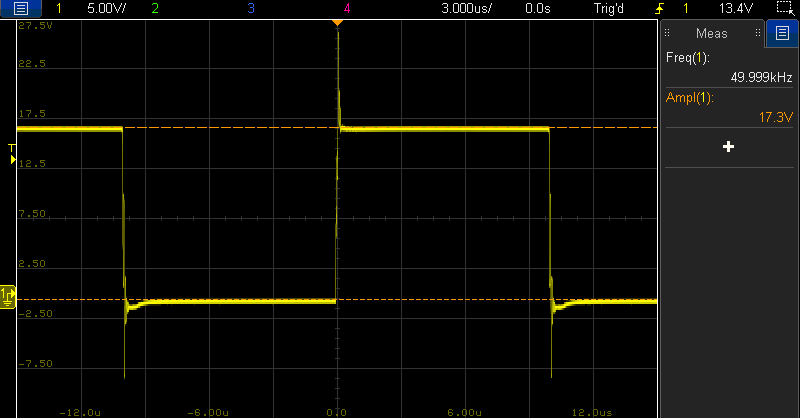
\includegraphics[width=0.6\linewidth]{images/scope_0.png}
    \caption{Segnale al gate del transistor}
    \label{fig:GateMeasure1}
\end{figure}
\begin{figure}[H]
    \centering
    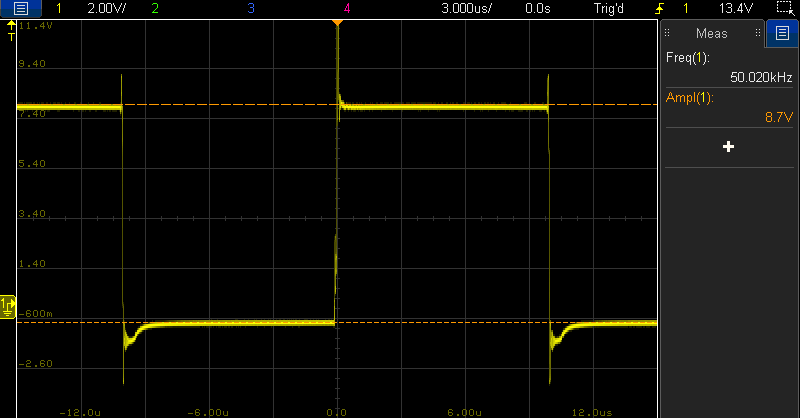
\includegraphics[width=0.6\linewidth]{images/scope_1.png}
    \caption{Segnale al source del transistor}
    \label{fig:SourceMeasure1}
\end{figure}
Come ci si aspetta, il segnale assume l'aspetto di un'onda quadra con frequenza di 50kHz.
\clearpage
In seguito è stata misurata la tensione di uscita ai capi della resistenza di carico $R$ come funzione del tempo, in Figura \ref{fig:OutputLoad1} è riportata la schermata dell'oscilloscopio.
\begin{figure}[H]
    \centering
    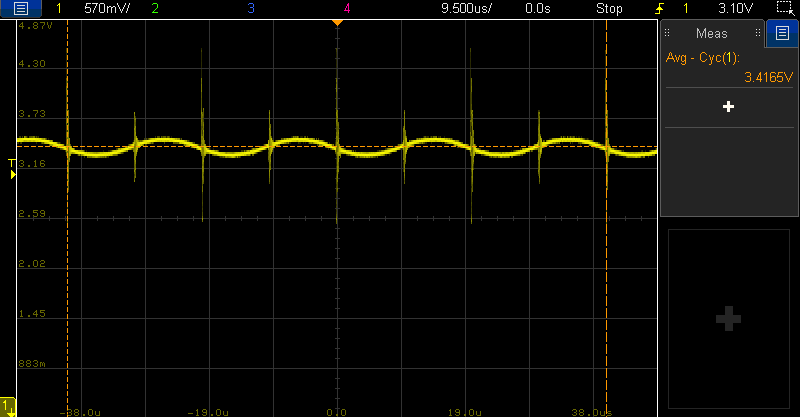
\includegraphics[width=0.6\linewidth]{images/scope_6.png}
    \caption{Tensione di uscita}
    \label{fig:OutputLoad1}
\end{figure}
In seguito è stato misurato anche il \textit{ripple} della tensione di uscita, sempre ai capi del carico $R$, riportato in Figura \ref{fig:OutputRipple1}. Si evidenzia che la misura del voltage ripple è stata eseguita impostando l'oscilloscopio in accoppiamento AC, in modo da eliminare le componenti continue del segnale di uscita.
\begin{figure}[H]
    \centering
    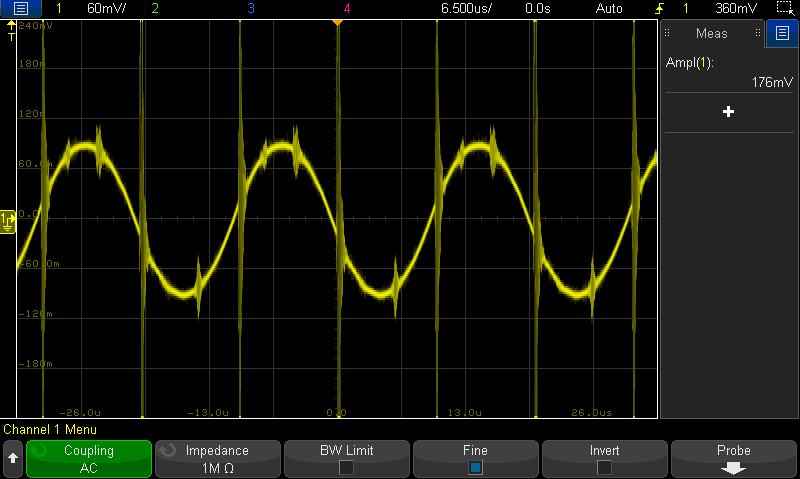
\includegraphics[width=0.6\linewidth]{images/scope_2.png}
    \caption{Apprezzamento del voltage ripple sul segnale di uscita}
    \label{fig:OutputRipple1}
\end{figure}
Si nota dal grafico in Figura \ref{fig:OutputLoad1} che la media della tensione di uscita calcolata dall'oscilloscopio è di $3.4165V$ che si discosta dal valore atteso di $V_0=\delta V_i=4V$. Dal grafico in Figura \ref{fig:OutputRipple1} si legge che il voltage ripple misurato è $176mV$ che è diverso dal valore di progetto ($100mV$). Entrambe queste anomalie sono dovute dapprima dalla configurazione a circuito aperto del circuito e in secondo luogo dalle tolleranze dei componenti utilizzati. Inoltre si osserva che il segnale presenta notevole disturbo.
\clearpage


\subsubsection{Misura della corrente sull'induttore}
Usando una sonda di corrente, è stata misurata la corrente che scorre nell'induttori durante pochi periodi di switching. Si riporta in Figura \ref{fig:CurrentInductor1} l'andamento della corrente misurato dall'oscilloscopio.
\begin{figure}[H]
    \centering
    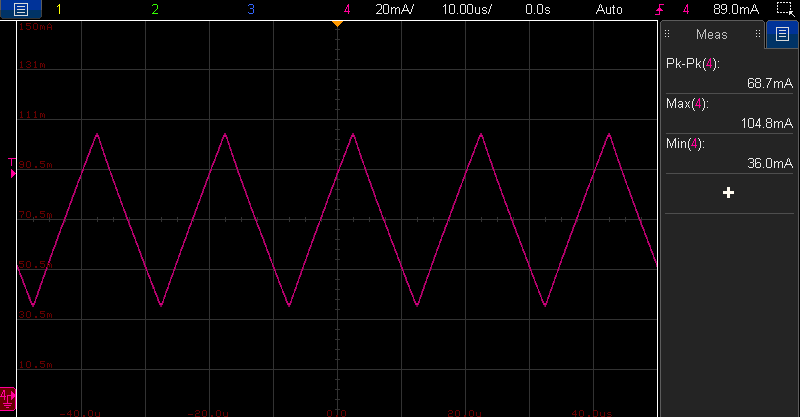
\includegraphics[width=0.8\linewidth]{images/scope_4.png}
    \caption{Corrente nell'induttore}
    \label{fig:CurrentInductor1}
\end{figure}
Infine si compara le misure delle correnti effettuate  con i valori teorici calcolati al punto \ref{ch:Cap1} ma con frequenza di duty cycle al 50\%
\begin{table}[H]
    \centering
    \begin{tabular}{|c|c|c|}
        \hline
        &Valore misurato&Valore teorico\\\hline\hline
        Corrente picco-picco&$68.7mA$&$58.8mA$\\\hline
        Corrente massima&$104.8mA$&$109.4mA$\\\hline
        Corrente minima&$36.0mA$&$50.6mA$\\\hline
    \end{tabular}
\end{table}
Anche qui si nota uno scostamento tra i valori teorici e i valori misurati. Per motivi già citati questi sono dovuti a tolleranze nelle componenti e alla configurazione a circuito aperto.
\clearpage
\subsubsection{Dipendenza tensione di uscita - duty cycle}
In conclusione dell'esperimento si vuole valutare la dipendenza tra la tensione di uscita e il duty cycle. In laboratorio è stata compilata la seguente Tabella \ref{tab:TabPlot}
\begin{table}[H]
    \centering
    \begin{tabular}{|c|c|}
        \hline
        Duty cycle (\%)&Output Voltage $V_o(V)$\\\hline\hline
        $20\%$&$1.0149V$\\\hline
        $30\%$&$1.8014V$\\\hline
        $40\%$&$2.6089V$\\\hline
        $50\%$&$3.4165V$\\\hline
        $60\%$&$4.2398V$\\\hline
        $70\%$&$5.0630V$\\\hline
        $80\%$&$5.2021V$\\\hline
    \end{tabular}
    \caption{Dati raccolti facendo variare il duty cycle del generatore}
    \label{tab:TabPlot}
\end{table}
Infine i dati sono stati plottati con l'ausilio di MATLAB ed è stato generato il diagramma in Figura \ref{fig:MatlabPlot1}
\begin{figure}[H]
    \centering
    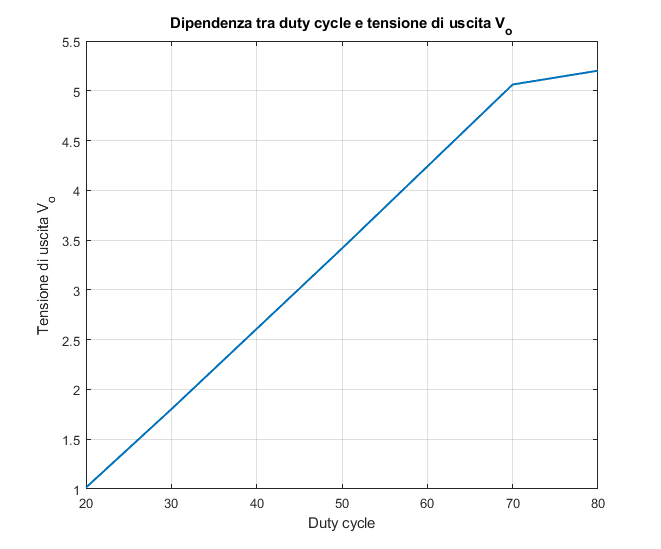
\includegraphics[width=0.7\linewidth]{images/Ris1TableDTCVo.png}
    \caption{Plot MATLAB dei dati raccolti in Tabella \ref{tab:TabPlot}}
    \label{fig:MatlabPlot1}
\end{figure}
Si nota che l'andamento, a parte un piccolo scostamento nella misura con duty cycle 80\%, è lineare. Come dopotutto ci si aspetta dalla relazione $V_o=\delta V_i$